\documentclass[10pt, letterpaper]{article}

\usepackage{amssymb,amsmath,amsfonts,eurosym,geometry,ulem,graphicx,caption,color,setspace,sectsty,comment,footmisc,caption,natbib,pdflscape,subfigure,array,hyperref}
\usepackage{xcolor}
\usepackage{mathptmx}
\usepackage{listings}
\lstset{language=Matlab}
\hypersetup{
    colorlinks,
    linkcolor={red!50!black},
    citecolor={blue!50!black},
    urlcolor={blue!80!black}
}
\normalem
\usepackage[flushleft]{threeparttable}
    
\onehalfspacing
\newtheorem{theorem}{Theorem}
\newtheorem{corollary}[theorem]{Corollary}
\newtheorem{proposition}{Proposition}
\newenvironment{proof}[1][Proof]{\noindent\textbf{#1.} }{\ \rule{0.5em}{0.5em}}

\newtheorem{hyp}{Hypothesis}
\newtheorem{subhyp}{Hypothesis}[hyp]
\newtheorem{asu}{Assumption}
\renewcommand{\thesubhyp}{\thehyp\alph{subhyp}}

\newcommand{\red}[1]{{\color{red} #1}}
\newcommand{\blue}[1]{{\color{blue} #1}}

\newcolumntype{L}[1]{>{\raggedright\let\newline\\arraybackslash\hspace{0pt}}m{#1}}
\newcolumntype{C}[1]{>{\centering\let\newline\\arraybackslash\hspace{0pt}}m{#1}}
\newcolumntype{R}[1]{>{\raggedleft\let\newline\\arraybackslash\hspace{0pt}}m{#1}}

\geometry{left=1.0in,right=1.0in,top=1.0in,bottom=1.0in}

\begin{document}

\title{Homework 2: ECON512}
\author{Joonkyo Hong}
\date{}
\maketitle
\smallskip

\noindent 1. 

\noindent The demands are determined by
\begin{align}
D_{A} = D_{B} = \frac{\exp(1)}{1+2\exp(1)} \nonumber
\end{align}
Matlab yields the following results:

\begin{verbatim}
D_A         D_B
0.42232     0.42232
\end{verbatim}

~\\

\noindent 2.

\noindent I start off with the initial guess $p^{0}=(1,1)'$. The criterion was 10e-08. With Broyden’s method, Matlab yields the following results:
\begin{verbatim}
iter 1: p(1) = 1.000000, p(2) = 1.000000, norm(f(x)) = 0.59724897
iter 2: p(1) = 0.577681, p(2) = 0.577681, norm(f(x)) = 0.96177748
iter 3: p(1) = 1.691933, p(2) = 1.691933, norm(f(x)) = 0.10363413
iter 4: p(1) = 1.583549, p(2) = 1.583549, norm(f(x)) = 0.01684145
iter 5: p(1) = 1.598700, p(2) = 1.598700, norm(f(x)) = 0.00026551
iter 6: p(1) = 1.598942, p(2) = 1.598942, norm(f(x)) = 0.00000069
iter 7: p(1) = 1.598942, p(2) = 1.598942, norm(f(x)) = 0.00000000
Equilibrium Prices
p_A         p_B
1.5989      1.5989
Computation Time
0.0062844
\end{verbatim}

~\\

\noindent 3. 

\noindent When I conduct Gauss-Seidel method to solve the problem, I start with two initial guesses $p^{0}=(2,2)'$ and $p^{-1}=(0,0)'$. The criterion was 10e-08. With this method, Matlab yields the following results:
\begin{verbatim}
iter 1: p(1) = 1.461030, p(2) = 1.567682, norm(f(x)) = 0.12757573
iter 2: p(1) = 1.591911, p(2) = 1.597363, norm(f(x)) = 0.00666873
iter 3: p(1) = 1.598588, p(2) = 1.598862, norm(f(x)) = 0.00033634
iter 4: p(1) = 1.598924, p(2) = 1.598938, norm(f(x)) = 0.00001691
iter 5: p(1) = 1.598941, p(2) = 1.598942, norm(f(x)) = 0.00000085
iter 6: p(1) = 1.598942, p(2) = 1.598942, norm(f(x)) = 0.00000004
Equilibrium Prices
p_A         p_B
1.5989      1.5989
Computation Time
0.016
\end{verbatim}
It took a longer time to solve the problem than the Broyden's method. The underlying logic of this solver comes from the rationalizability in game theory while Broyden's method solves for a price vector in line with the logic of Nash-equilibrium. As it is easier to solve for equilibrium with Nash equilibrium than with rationalizability, it is not that surprising that Broyden's method is 
faster than this method.

~\\

\noindent 4.

\noindent I also start with $p=(1,1)'$. Under the parametrization $v=(2,2)'$, the proposed updating rule successfully found the root and it was the fastest one among three methods. Matlab yields the following results:
\begin{verbatim}
iter 1: p(1) = 1.000000, p(2) = 1.000000, norm(f(x)) = 1.03387296
iter 2: p(1) = 1.731059, p(2) = 1.731059, norm(f(x)) = 0.23225003
iter 3: p(1) = 1.566833, p(2) = 1.566833, norm(f(x)) = 0.05628097
iter 4: p(1) = 1.606630, p(2) = 1.606630, norm(f(x)) = 0.01348578
iter 5: p(1) = 1.597094, p(2) = 1.597094, norm(f(x)) = 0.00324129
iter 6: p(1) = 1.599386, p(2) = 1.599386, norm(f(x)) = 0.00077848
iter 7: p(1) = 1.598835, p(2) = 1.598835, norm(f(x)) = 0.00018701
iter 8: p(1) = 1.598967, p(2) = 1.598967, norm(f(x)) = 0.00004492
iter 9: p(1) = 1.598936, p(2) = 1.598936, norm(f(x)) = 0.00001079
iter 10: p(1) = 1.598943, p(2) = 1.598943, norm(f(x)) = 0.00000259
iter 11: p(1) = 1.598942, p(2) = 1.598942, norm(f(x)) = 0.00000062
iter 12: p(1) = 1.598942, p(2) = 1.598942, norm(f(x)) = 0.00000015
iter 13: p(1) = 1.598942, p(2) = 1.598942, norm(f(x)) = 0.00000004
Equilibrium Prices
p_A         p_B
1.5989      1.5989
Computation Time
0.005888
\end{verbatim}

\noindent However, the method is highly sensitive to parametrization. For instance, under $v=(2,3)'$, the method fails to find the fixed point (Even start with $p=(1,2)'$ which is close to the solution). 
\begin{verbatim}
...
iter 995: p(1) = 1.023864, p(2) = 7.133538, norm(f(x)) = 6.65331409
iter 996: p(1) = 3.612315, p(2) = 1.004386, norm(f(x)) = 6.65331409
iter 997: p(1) = 1.023864, p(2) = 7.133538, norm(f(x)) = 6.65331409
iter 998: p(1) = 3.612315, p(2) = 1.004386, norm(f(x)) = 6.65331409
iter 999: p(1) = 1.023864, p(2) = 7.133538, norm(f(x)) = 6.65331409
iter 1000: p(1) = 3.612315, p(2) = 1.004386, norm(f(x)) = 6.65331409
Equilibrium Prices
p_A         p_B
1.0239      7.1335
Computation Time
0.067707
\end{verbatim}


~\\


\noindent 5.

\noindent The generated figures are as follow.

\begin{figure}[!h]
\begin{center}
  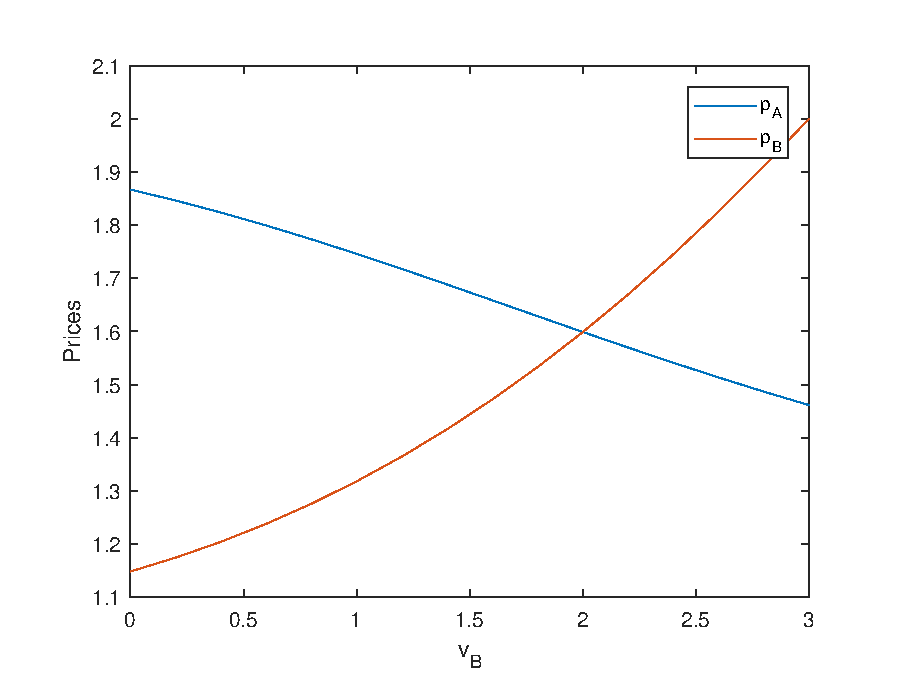
\includegraphics[width=\linewidth]{figure.eps}
  \caption{}
  \label{fig:graph}
\end{center}
\end{figure}


\clearpage

\begin{verbatim}
%%%%%%%%%%%%%%%%%%%%%%%%%%%%%%%%%%%%%%%%%%%%%%%%%%%%%%%%%%%
% Homework #2 ECON 512                                    %
% Written by Joonkyo (Jay) Hong, 20 Sept 2018             %
%%%%%%%%%%%%%%%%%%%%%%%%%%%%%%%%%%%%%%%%%%%%%%%%%%%%%%%%%%%
clear;

%% Question 1

v=[2;2];
p=[1;1];

demand = exp(v-p)./(1+sum(exp(v-p)));

disp('D_A         D_B')
disp(num2str(demand'));
disp("Question 1 is done. Press any key to continue");
pause
%% Question 2

f = @(p) bertrand(p,v); %make function handle whose argument is a price vector
                        %Bertrand is an outside function that characterize
                        %equilibrium conditions

% START BROYDEN METHODS

maxiter = 100;
tol = 10e-8;

% initial guess
p = [1;1];

init_f = f(p);
invJ = eye(length(p));

tic
 for i=1:maxiter
      fnorm = norm(init_f);
      fprintf('iter %d: p(1) = %f, p(2) = %f, norm(f(x)) = %.8f\n', i, p(1), p(2), fnorm);
      if fnorm < tol
          break;
      end
      
      d = - (invJ*init_f);
      p = p + d;
      new_f = f(p);
      u = invJ*(new_f - init_f);
      invJ = invJ + ( (d - u) * (d'*invJ) )/ (d'*u);
      
      init_f = new_f;
 end
t=toc;

disp("Equilibrium Prices")
disp('p_A         p_B')
disp(num2str(p'));
disp("Computation Time")
disp(num2str(t));
disp("Question 2 is done. Press any key to continue");
pause

%% Question 3

pa = 1; pb=1;

f = @(p) bertrand(p,v); % Again, make function handle
fval = f([pa;pb]);
pa_old = 0;
pb_old = 0;
bigloop_iter = 1000;

tic

for i=1:bigloop_iter % Big loop
    if norm(fval) < 10e-8    
        break
    end

% Sub loop for good A 
% In order to perform secent method, fix two initial conditions

      fa = @(pa) bertrand1(pa,pb,v);   % FOC only for good A
      faold = fa(pa_old);

      maxiter = 100;
      tol = 10e-8;

      for j=1:maxiter
          faval = fa(pa);
          if norm(faval) < tol
             break
          else
             pa_new = pa - ( (pa - pa_old)/(faval-faold) )*faval;
             pa_old = pa;
             pa = pa_new;
             faold = faval;
          end
      end

% Sub loop for good B

       fb = @(pb) bertrand2(pa,pb,v);
       fbold = fb(pb_old);

     for j=1:maxiter
          fbval = fb(pb);
         if norm(fbval) < tol
            break
         else
            pb_new = pb - ( (pb - pb_old)/(fbval-fbold) )*fbval;
            pb_old = pb;
            pb = pb_new;
            fbold = fbval;
         end
     end
 
     fval=f([pa;pb]);     % Updating fval for the next loop
     fprintf('iter %d: p(1) = %f, p(2) = %f, norm(f(x)) = %.8f\n',i, pa, pb, norm(fval));
     
end
t=toc;

disp("Equilibrium Prices")
disp('p_A         p_B')
disp(num2str([pa pb]));
disp("Computation Time")
disp(num2str(t));
disp("Question 3 is done. Press any key to continue");
pause
%% Question 4

% Updating Rule

g = @(p) 1./(1 - exp(v-p)./(1+sum(exp(v-p))));

p = [1;1];

maxit = 1000;

tic
 for i=1:maxit
     nextp = g(p);
     diff = norm(nextp-p);
     fprintf('iter %d: p(1) = %f, p(2) = %f, norm(f(x)) = %.8f\n',i, p(1), p(2), diff);
      if diff < 10e-8
          break;
      end
      p = nextp;
 end
t=toc;

% What if v2=3?

v = [2;3];
g = @(p) 1./(1 - exp(v-p)./(1+sum(exp(v-p))));

p2 = [1;2];

maxit = 1000;

tic
 for i=1:maxit
     nextp2 = g(p2);
     diff = norm(nextp2-p2);
     fprintf('iter %d: p(1) = %f, p(2) = %f, norm(f(x)) = %.8f\n',i, p2(1), p2(2), diff);
      if diff < 10e-8
          break;
      end
      p2 = nextp2;
 end
t2=toc;

disp("CASE 1: v1=v2=2")
disp("Equilibrium Prices")
disp('p_A         p_B')
disp(num2str(p'));
disp("Computation Time")
disp(num2str(t));
disp("Question 4 is done. Press any key to continue");

disp(" ")

disp("CASE 2: v1=2, v2=3")
disp("Equilibrium Prices")
disp('p_A         p_B')
disp(num2str(p2'));
disp("Computation Time")
disp(num2str(t2));
disp("Question 4 is done. Press any key to continue");

pause
%% Question 5

vb_vec = 0:0.2:3;                        % vector of values 
p_eqmvec = zeros(length(vb_vec),2);      % vector that will contain the equilibrium prices
p = [1;1];                               % Initial guess of solution 


for iter=1:length(vb_vec)   
    
    vb = vb_vec(iter);
    v = [2;vb];
    f = @(p) bertrand(p,v);    
    
          % Perform Broyden Method to solve the equilibrium
          
          init_f = f(p);
          invJ = eye(length(p)); 
          maxiter = 1000;
          tol = 10e-8;
              
             for i=1:maxiter
                 fnorm = norm(init_f);
                 
                 if fnorm < tol
                     break;
                 end
                 
                 d = - (invJ*init_f);
                 p = p + d;
                 new_f = f(p);
                 u = invJ*(new_f - init_f);
                 invJ = invJ + ( (d - u) * (d'*invJ) )/ (d'*u);
                 
                 init_f = new_f;
             end
            
        
        p_eqmvec(iter,:) = p';
    
end

figure(1)
plot(vb_vec,p_eqmvec);
xlabel('v_{B}');
ylabel('Prices');
legend('p_{A}', 'p_{B}');
disp("Question 5 is done. See the figure that poped up");
\end{verbatim}
                     

\end{document}